\documentclass[aps,prx,reprint,superscriptaddress,footnote, twocolumn,notitlepage]{revtex4-2}

%\usepackage[T1]{fontenc}
%\usepackage[utf8x]{inputenc}
%\usepackage[sc,osf]{mathpazo}\linespread{1.05}
\usepackage{amsmath, amsthm, amssymb,amsfonts,mathbbol,amstext}
\usepackage{braket}
\usepackage{pifont}
\usepackage{graphicx}
\usepackage{dcolumn}
\usepackage{bm}
\usepackage{bbm}
\usepackage{hyperref}
\usepackage{mathtools}
\usepackage{comment}
\usepackage{color}
\usepackage{multirow}
\usepackage{diagbox}
\usepackage{float}
\usepackage{xcolor}
\usepackage{makecell}
\usepackage[normalem]{ulem}
\usepackage{soul}
\newcommand{\yu}[1]{\textcolor{blue}{#1}}
\newcommand{\tom}[1]{\textcolor{green}{#1}}
\newcommand{\ko}[1]{\textcolor{orange}{#1}}
\newcommand{\ph}[1]{\textcolor{purple}{#1}}


\newcommand{\todoyu}[1]{\yu{$\heartsuit$ #1}}
\newcommand{\todotom}[1]{\tom{$\spadesuit$ #1}}
\newcommand{\todoko}[1]{\ko{$\diamondsuit$ #1}}
\newcommand{\todoph}[1]{\ph{$\clubsuit$ #1}}

% Language setting
% Replace `english' with e.g. `spanish' to change the document language
\usepackage[english]{babel}

% Set page size and margins
% Replace `letterpaper' with `a4paper' for UK/EU standard size
\usepackage[letterpaper,top=2cm,bottom=2cm,left=3cm,right=3cm,marginparwidth=1.75cm]{geometry}

% Useful packages
\usepackage{amsmath}
\usepackage{graphicx}
% \usepackage[colorlinks=true, allcolors=blue]{hyperref}

\begin{document}
\title{Look Mum No Hands: Reachability in Autonomous Quantum Systems}


\author{Tomasz Andrzejewski}
\email{tomasz.andrzejewski@tuwien.ac.at}
\affiliation{Atominstitut, Technische Universit{\"a}t Wien, Stadionallee 2, 1020 Vienna, Austria}

\author{Yuri Minoguchi}
\affiliation{Atominstitut, Technische Universit{\"a}t Wien, Stadionallee 2, 1020 Vienna, Austria}


\author{Phila Rembold}
\affiliation{Atominstitut, Technische Universit{\"a}t Wien, Stadionallee 2, 1020 Vienna, Austria}

\author{Konrad Szymanski}
\email{k.sz@quantumstat.es}
\affiliation{Research Center for Quantum Information, Slovenská Akadémia Vied, Dúbravská cesta 9, 84511 Bratislava, Slovakia}
\affiliation{Naturwissenschaftlich-Technische Fakultät, Universität Siegen, Walter-Flex-Straße 3, 57068 Siegen, Germany}


\begin{abstract}
Things to do (feel free to pick yr color):\\
\todoko{Konrad}\\
\todotom{Tomek}\\
\todoyu{Yuri}\\
\todoph{Phila}
\end{abstract}


\maketitle
\section{Introduction}
\subsection{Motivation}
\todoyu{From Phila: Yuri, please have a look and feel free to change anything around}\\
Precise control is what turns theoretical advantages into technologies.
A quantum system can only be explored to its full capacity, if we possess the tools to navigate between any two points of its Hilbert space.
In the context of optimal control, a system is called controllable, if any state can be reached in finite time using a set of time-dependent controls.
However, what if these controls are static, i.e., fixed in time?
We define autonomous quantum systems by their lack of time-dependent operations: They evolve under their own Hamiltonian in their self-contained state space.
As such, all they require is calibration, i.e., the careful setup of the Hamiltonian ahead of time, to ultimately end up in the desired state.
On the experimental side, the autonomous reachability describes the versatility of a system where controls are only switched on and off once rather than changed continuously. 
This approach can also be seen as a shaping of the energy landscape~\cite{schirmer_design_2018} leading the system from the initial to the final state. 
While the method provides a simplified control protocol compared to its dynamical counterparts, it has also been shown to exhibit provable robustness \todoph{check  [14-16] of \cite{schirmer_design_2018}}.
Explicit control protocols have been constructed theoretically for spin chains~\cite{schirmer_design_2018} and experimentally for atoms in optical lattices~\cite{weidner_energy_2025}. \todoph{insert more refs, possibly expand?}

Moreover, recent work implies that any time-dependent control can be replaced with a time-independent version using auxiliary systems~\cite{mooney_time_2025}.
Finally, the autonomous framework is at the base of autonomous quantum thermal machines~\cite{meier_autonomous_2024}---a fully self-contained description of quantum computing leveraged to derive its fundamental thermodynamics limits.
\todoph{Find more references and check that definition is correct} \todoko{Find Sophie Schermer and Gdańsk group papers}

\begin{itemize}
    \item energy landscape optimization 
    \item autonomus quantum machine 
    \item \yu{some stuff}
\end{itemize}

\begin{figure}
    \centering
    \includegraphics[width=0.9\linewidth]{Hilbert.png}
    \caption{Dependent on the set of Hamiltonians, only part of the Hilbert space is reachable. The portion depends on the given set.}
    \label{fig:hilbert}
\end{figure}

\section{Main part }
\subsection{Preliminaries, proper math, setup}
\subsection{Analyzed systems}\label{sec:systems}
\subsubsection{\yu{Qudits with canonized basis of Hamiltonians}}
\label{sec:canonical}

The canonical basis provides a complete orthogonal basis for $d\times d$ Hermitian matrices. For a $d$-dimensional Hilbert space, the basis operators are defined as:
\begin{equation}
\begin{aligned}
X_{jk} &= |j\rangle\langle k| + |k\rangle\langle j| \quad (j < k), \\
Y_{jk} &= -i|j\rangle\langle k| + i|k\rangle\langle j| \quad (j < k), \\
Z_j &= |j\rangle\langle j| - |j+1\rangle\langle j+1| \quad (j = 0, \ldots, d-2), \\
I &= \mathbb{1}_d,
\end{aligned}
\label{eq:canonical_basis}
\end{equation}
where indices run over $j, k \in \{0, \ldots, d-1\}$. This gives $d^2$ operators total: $d(d-1)/2$ operators each for $X$ and $Y$ types, $(d-1)$ operators of $Z$ type, and the identity. 


 \subsubsection{\todotom{Geometric 2-local}} \label{sec:geo2}
 We also test our criteria on the geometric 2-local (GEO2Local) ensemble~\cite{quek2025quantumadvantagerandomgeometricallytwolocal} relevant for quantum computing hardware.
It consists of geometrically 2-local Pauli operators on a graph $G = (V, E)$ with $n = |V|$ qubits. The Hamiltonian is drawn from the Gaussian distribution
\begin{equation}
H(\mathbf{g}) = \frac{1}{\sqrt{|\mathcal{P}_2|}} \sum_{P \in \mathcal{P}_2} g_P P, \quad g_P \stackrel{\text{i.i.d.}}{\sim} \mathcal{N}(0, 1),
\label{eq:geo2local_general}
\end{equation}
where $\mathcal{P}_2$ is the set of Pauli strings of locality at most $k=2$ (acting on at most 2 qubits within graph distance $\leq 2$), and $|\mathcal{P}_2|$ is the total operator count. The set $\mathcal{P}_2$ contains:
\begin{itemize}
\item \emph{1-local terms}: $\{X_i, Y_i, Z_i\}$ for all sites $i \in V$, contributing $3n$ operators.
\item \emph{2-local terms}: $\{X_i X_j, X_i Y_j, \ldots, Z_i Z_j\}$ for all edges $(i,j) \in E$ with lattice distance $d_{\text{lattice}}(i,j) \leq 2$, contributing $9|E|$ operators.
\end{itemize}
The total operator count is $|\mathcal{P}_2| = L = 3n + 9|E|$. Following ~\cite{quek2025quantumadvantagerandomgeometricallytwolocal} we will consider rectangular 2D lattice with $n = L_x \times L_y$ sites with nearest-neighbor connectivity, for which $|E| = 2L_x L_y - L_x - L_y$. \ko{Note that for interactions spanned only by the 2-local terms $\{X_i X_j+Y_iY_j, X_iY_j-Y_iX_j,Z_iZ_j\}$ and 1-local $\{Z_i\}$ conserve the total excitation number $
\sum Z_i$, and in the 1-excitation subspace they reduce to the canonical basis of qudit Hamiltonians \cite{wang_symmetry_2012,schirmer_design_2018}.}


\textbf{Example: Transverse-Field Ising Model.} I think the nearest-neighbor transverse-field Ising Hamiltonian
\begin{equation}
H_{\text{TFIM}} = -J \sum_{\langle i,j \rangle} Z_i Z_j - h \sum_i X_i
\end{equation}
is a special case of Eq.~\eqref{eq:geo2local_k2} with $k=1$ locality (nearest neighbors only), using only $ZZ$ and $X$ terms. 


\ko{TODO: Answer questions below}
\textbf{Question 1:}
For optimization, I guess we need to reparameterize Eq.~\eqref{eq:geo2local_general} with control parameters $\lambda \in \mathbb{R}^L$ instead of Gaussian coefficients giving
% \begin{equation}
% H(\lambda) = \sum_{i \in V} \sum_{\alpha \in \{X,Y,Z\}} \lambda_{i,\alpha} \sigma_i^\alpha
%            + \sum_{\substack{(i,j) \in E \\ d(i,j) \leq 2}} \sum_{\alpha,\beta \in \{X,Y,Z\}} \lambda_{ij,\alpha\beta}
%              \sigma_i^\alpha \otimes \sigma_j^\beta,
% \label{eq:geo2local_k2}
% \end{equation}

\begin{equation}
\begin{aligned}
H(\lambda) = \sum_{i \in V} \sum_{\alpha \in \{X,Y,Z\}} \lambda_{i,\alpha} \sigma_i^\alpha \\
           + \sum_{\substack{(i,j) \in E \\ d(i,j) \leq 2}} \sum_{\alpha,\beta \in \{X,Y,Z\}} \lambda_{ij,\alpha\beta} \sigma_i^\alpha \otimes \sigma_j^\beta
\end{aligned}
\label{eq:geo2local_k2}
\end{equation}
where $\sigma^\alpha$ denotes the Pauli matrix for $\alpha \in \{X, Y, Z\}$.


\textbf{Question 2: Dimension} The GEO2Local ensemble is qubit-based, with each lattice site occupied by a $d=2$ dimensional quantum system. The total Hilbert space dimension grows exponentially as $\dim(\mathcal{H}) = 2^{n}$ with lattice size $n = L_x \times L_y$. This differs from the canonical basis ensemble (Section~\ref{sec:canonical}), which explores a \emph{single} qudit of dimension $d \in \{8, 10, \ldots, 16\}$ with Hilbert space dimension $\dim(\mathcal{H}) = d$. While we can use control density $\rho = K/d^2$ in plots for both ensembles, the meaning of ``$d$'' will differ: for canonical basis, $d$ is the qudit dimension; for GEO2Local, $d = 2^n$ is the exponentially-large total Hilbert space dimension. \todotom{Would such plots make sense?} Then I guess with GEO2Local and canonical ensemble we would  explore complementary physical regimes: \emph{many weakly-coupled qubits under geometric constraints} versus \emph{a single strongly-interacting qudit}. 

\textbf{Motivation: Computational complexity and quantum learning.} The GEO2Local ensemble was introduced in~\cite{quek2025quantumadvantagerandomgeometricallytwolocal} to study the complexity of $\varepsilon$-sampling and $\varepsilon$-emulation tasks \todoyu{(what exactly are they though?) explain them} under geometric constraints. Related work~\cite{park2023hardnessquantumspindynamics} has established that sampling from output distributions of geometrically local Hamiltonians (including Ising, XX, and Heisenberg models) is classically intractable on 2D lattices. Our reachability analysis aims to quantify these limits: the critical control density $\rho_c(\tau)$ and threshold-dependent transition width $\Delta(\tau)$ determine the resource requirements (number of Hamiltonian terms $K$) needed to reach target states with fidelity $> \tau$. This should tell us about the achievability of $\varepsilon$-approximation tasks, where $\varepsilon \sim 1 - \tau$, providing a state-space perspective on approximation capabilities of geometrically constrained Hamiltonians.
\subsubsection{\yu{GUE?}}
\ko{Let's finish qudits/hopping particles first. I believe Krylov criterion is not compatible with this, since generically the subspace has full dimension.}
\subsection{Criteria}

%Defining an initial state $\ket{\phi}$, we will call a state reachable, if it can be described by $\ket{\phi(t)}=\exp\left(-i H t \right)\ket{\phi}$, where $H=\sum_n^k \lambda_n H_n$ for a specified set of generators $\{H_1,\ldots, H_k\}$. 
%Extending that description, we generally call a state $\ket{\psi}$ reachable, if it lies  within a given distance $\varepsilon>0$ from $\ket{\phi(t)}$. \footnote{For instance, every state $\ket{\psi'}=\frac{1}{\sqrt3} \left(\ket{0}+e^{i\alpha }\ket{1} +e^{i\beta} \ket{2}\right)$ is reachable from $\ket{\phi}=\frac{1}{\sqrt3} \left(\ket{0}+\ket{1} +\ket{2}\right)$ with the Hamiltonian $H=\ket{1}\bra{1}+\sqrt{2}\ket{2}\bra{2}$ in the latter sense, but not the former.} 

%Considering the commutation relation $\left[H,e^H\right]=0$, we can find properties any reachable state $\ket{\psi}$ possesses.
%If a given state does not match one of these properties it is hence unreachable, which is often simpler to check than the opposite.

%In this section, we will write expectation values $\bra{\alpha}A\ket{\alpha}=\langle A \rangle_\alpha$ for brevity.

Consider an initial state $\ket{\phi}$ evolving under a Hamiltonian $H = \sum_{n=1}^{k} \lambda_n H_n$, where $\{H_1, \ldots, H_k\}$ is a fixed set of generators and the $\lambda_n$ are real parameters. The time evolution yields $\ket{\phi(t)} = \exp(-iHt)\ket{\phi}$. We call a state $\ket{\psi}$ \emph{reachable} from $\ket{\phi}$ if it lies in the closure of such orbits, meaning $\ket{\psi}$ can be approached arbitrarily closely by some $\ket{\phi(t)}$.\footnote{In finite dimensions, this accounts for situations analogous to irrational winding on a torus, where an orbit comes arbitrarily close to certain states without ever reaching them exactly. For instance, every state $\ket{\psi'} = \frac{1}{\sqrt{3}}(\ket{0} + e^{i\alpha}\ket{1} + e^{i\beta}\ket{2})$ is reachable from $\ket{\phi} = \frac{1}{\sqrt{3}}(\ket{0} + \ket{1} + \ket{2})$ with Hamiltonian $H = \ket{1}\bra{1} + \sqrt{2}\ket{2}\bra{2}$ in this sense, though only a measure-zero subset can be reached exactly.}

We denote the eigenstates of $H$ by $\ket{\alpha_i}$, with $H\ket{\alpha_i} = E_i\ket{\alpha_i}$. Generically, unless the generators $H_n$ possess special structure (such as shared symmetries), the only conserved quantities are functions of $H$ itself. Since $[H, f(H)] = 0$ for any function $f$, any such conserved quantity constrains which final states $\ket{\psi}$ are reachable. Checking whether a candidate state violates one of these conservation laws is often simpler than directly verifying reachability. Throughout this section, we write $\braket{A}_\alpha = \bra{\alpha}A\ket{\alpha}$ for expectation values.

We now present three criteria for deciding whether a state $\ket{\psi}$
 is reachable from $\ket{\phi}$ via a Hamiltonian drawn from a specified family.
%\todoko{You might want to adapt this to make it more focused on reachability, feel free to change everything}
\subsubsection{\ko{Moment criterion}}

Since the Hamiltonian commutes with its own exponential, all moments $\langle H^m \rangle$ are conserved under time evolution:
\begin{equation}
    \langle H^m \rangle_{\phi(t)} = \langle e^{iHt} H^m e^{-iHt} \rangle_\phi = \langle H^m \rangle_\phi.
\end{equation}
Consequently, if $\ket{\psi}$ is reachable from $\ket{\phi}$, the two states must share all moments of the Hamiltonian.\footnote{For states that lie on the orbit, this is immediate. For states in the closure of the orbit, conservation follows from continuity of the expectation value, which holds in finite dimensions.} The case $m=1$ corresponds to energy conservation.

Recall that we are interested in whether \emph{any} Hamiltonian from the family $H = \sum_n \lambda_n H_n$ can connect $\ket{\phi}$ to $\ket{\psi}$. Conservation of the first moment requires
\begin{equation}
    L := \sum_n \lambda_n \left( \langle H_n \rangle_\phi - \langle H_n \rangle_\psi \right) = 0.
    \label{eq:first_moment}
\end{equation}
By itself, this constraint is not very useful: as long as some generators have $\langle H_n \rangle_\phi \neq \langle H_n \rangle_\psi$, we can always find weights $\lambda_n$ that make $L$ positive, negative, or zero. The first moment alone cannot rule out reachability.

The second moment provides a stronger constraint. Defining
\begin{equation}\begin{aligned}
    Q &:= \langle H^2 \rangle_\phi - \langle H^2 \rangle_\psi \\
    &= \sum_{n,m} \lambda_n \lambda_m \left( \langle \{H_n, H_m\} \rangle_\phi - \langle \{H_n, H_m\} \rangle_\psi \right),
    \end{aligned}
\end{equation}
where $\{A, B\} = AB + BA$ denotes the anticommutator, we require $Q = 0$ for any reachable state. As with Eq.~\eqref{eq:first_moment}, this condition alone can often be satisfied by a suitable choice of weights. However, requiring \emph{both} $L = 0$ and $Q = 0$ simultaneously is more restrictive.

To formalize this, consider the quadratic form
\begin{equation}
    M(\gamma) = Q + \gamma L^2 = \sum_{n,m} M_{nm} \lambda_n \lambda_m,
\end{equation}
where $M_{nm}$ is a real symmetric matrix determined by $\gamma$ and the expectation values of generators and their anticommutators. If $M(\gamma)$ is strictly positive definite (or strictly negative definite) for some choice of $\gamma$, then no non-trivial weights $\lambda_n$ can make both $L$ and $Q$ vanish. Since the trivial choice $\lambda_1 = \cdots = \lambda_k = 0$ generates no dynamics, this certifies that $\ket{\psi}$ is unreachable from $\ket{\phi}$ using any Hamiltonian in the family.

This criterion is straightforward to apply: it requires only the expectation values of the generators $H_n$ and their anticommutators over the states of interest, followed by checking whether a matrix is positive definite~\footnote{The latter is numerically well-behaved, as eigenvalue computations are stable and the result is unambiguous unless eigenvalues are extremely close to zero.}. The limitation is that the test is one-sided: it can certify unreachability, but passing the test does not guarantee that $\ket{\psi}$ is reachable. For more refined analysis, one can extend to higher moments or optimize over the Hamiltonian family directly, though such approaches are more computationally involved and offer weaker mathematical guarantees.

\begin{comment}

The moments of a state do not change as it evolves freely, as proven by the fact that a fixed Hamiltonian commutes with its exponent:
%To make this more explicit, we can check for the first two moments.
%The expectation value for the full Hamiltonian gives
\begin{equation}
    %\begin{split}
        \langle H^m\rangle_{\phi(t)}=\langle e^{iHt}H^me^{-iHt}\rangle_\phi\\
        =\langle H^m\rangle_\phi,\\
   % \end{split}
\end{equation}
which for $m=1$ is equivalent to energy conservation. Therefore, if a state $\ket\psi$ is reachable the following expression vanishes:
\begin{equation}
    L=\sum_n \lambda_n(\langle H_n\rangle_\phi-\langle H_n\rangle_\psi).
\end{equation}
Similarly, for $m=2$, a similar expression can be defined capturing the conservation of the second moment of the Hamiltonian. Here, $Q$, as defined below, must vanish for any reachable state.
\begin{equation}
    \begin{split}
        Q&=\langle H^2\rangle_\phi-\langle H^2\rangle_\psi \\
        &= \sum_{n,m} \lambda_n \lambda_m \left(\langle\{H_n,H_m\}\rangle_\psi-\langle\{H_n,H_m\}\rangle_\phi\right),
    \end{split}
\end{equation}
where $\{A,B \}=AB+BA$ denotes the anticommutator. 

In general, this list can be extended to arbitrary moments, resulting in the criteria $\langle H^m\rangle_\psi - \langle H^m \rangle_\phi=0$ for all $m$. 
As a result, a state is only reachable with the given set of generators, $H_n$, if there exists a set of weights $\{\lambda_n\}$ for which all of the criteria are met. 

In some cases there may exist no assignment of weights $\{\lambda_n\}$ other than $\lambda_1=\ldots=\lambda_n=0$ for which first and second moments coincide (and zero weights generate no dynamics). To make things concrete, if 
\begin{equation}
    M(\alpha) = Q+\alpha L^2 =\sum M_{m,n} \lambda_n \lambda_n,
\end{equation}
is strictly positive definite (the real symmetric matrix $M_{m,n}$ has only strictly positive eigenvalues) for some choice of $\alpha$, this means that for no $\lambda_n$ both $Q$ and $L$ can be made zero (except the trivial case, which generates no dynamics). The same applies if $M_{m,n}$ is strictly negative definite.

The above criterion is easy to apply, as it depends only on expectation values of the generators $H_n$ and their anticommutators over the states of interest. However, it is also relatively restricted: the possible outcomes are that a state is unreachable or the test is insufficient to decide. On the upside, except for matrix diagonalization, no numerics or optimization is necessary. For more fine-grained, but less mathematically grounded tests we need to look into more moments -- or probabilities of finding the eigenstates, and numerically optimize over the Hamiltonian family directly. 
\end{comment}
\subsubsection{\ko{Spectral overlap criterion}}
Any state that is not an eigenstate of the Hamiltonian will evolve, but its decomposition in terms of eigenstates changes only by phases. \ko{This observation was first used in \cite{schirmer_design_2018} to obtain a bound for distance between the target state and an orbit generated by a fixed Hamiltonian.}
Fix a nondegenerate Hamiltonian $H$ with eigenstates $\ket{\alpha_i}$ and eigenvalues $E_i$, and decompose the initial state as
\begin{equation}
    \ket{\phi} = \sum_i \sqrt{p_i} \ket{\alpha_i},
\end{equation}
where we have absorbed any phases into the definition of the eigenstates. The probabilities $p_i = |\langle \alpha_i | \phi \rangle|^2$ are invariant under evolution generated by $H$.

For a target state $\ket{\psi} = \sum_i \sqrt{q_i} e^{i\theta_i} \ket{\alpha_i}$, the distance to the orbit of $\ket{\phi}$ is bounded from below\footnote{\textbf{[TODO: add proof]}}:
\begin{equation}
    \inf_{t \in \mathbb{R}} \| \ket{\phi(t)} - \ket{\psi} \| \geq C \sum_i |p_i - q_i|,
\end{equation}
for dimension-dependent constant $C > 0$. Reachability therefore requires $p_i = q_i$ for all $i$.

This motivates the spectral overlap criterion. Define
\begin{equation}
    S(\ket{\phi}, \ket{\psi}, H) = \sum_i \sqrt{p_i q_i} = \sum_i |\langle \psi | \alpha_i \rangle| \, |\langle \alpha_i | \phi \rangle|,
\end{equation}
which equals 1 if and only if the two probability distributions coincide. We numerically optimize $S$ over the Hamiltonian family $H = \sum_n \lambda_n H_n$. If the maximum value of $S$ falls below $1 - \varepsilon$ for a chosen tolerance $\varepsilon$, the state is deemed unreachable. \todoko{[TODO: current plots use $\varepsilon = 0.05$; reduce to $\varepsilon = 0.01$ , what are the typical thresholds in quantum control anyway?]}

Unlike the moment criterion, the spectral criterion requires numerical optimization over the parameters $\lambda_n$, which may converge to local maxima and does not provide a certificate of correctness. However, it offers a more fine-grained test: rather than checking polynomial constraints on expectation values, it directly examines whether the spectral distributions can be made to match. One advantage is that optimization is only over the Hamiltonian parameters, not over time, since the probabilities $p_i$ and $q_i$ are time-independent.

\begin{comment}
Any quantum state that is not an eigenstate of the Hamiltonian will evolve. 
However, its decomposition in terms of eigenstates does not change, only the phases between them. Let us fix the Hamiltonian $H$, and look at the decomposition of the initial state $\ket\phi$ in the eigenbasis of $H$ (assuming nondegenerate):
\begin{equation}
    \ket\phi=\sum \sqrt{p_n} \ket{n},~H\ket{n}=E_n\ket{n}.
\end{equation}
The distance of any target state $\ket\psi=\sum \sqrt{q_n}e^{i\theta_n}\ket{n}$ to the orbit of $\ket\phi$ under evolution generated by $H$ is bounded from below: \ko{(it's somewhere in my notes, need to dig it up)}:
\begin{equation}
    \sup_{t\in\mathbb{R}} \lvert \ket{\phi(t)}-\ket\psi\rvert \ge \text{const}\times \sum \lvert p_n-q_n\lvert.
\end{equation}
Therefore, reachability can only happen if $p_n=q_n$. Maximization of the overlap of the two probability distributions is the goal of the spectral criterion:
\begin{equation}
    S(\ket\phi,\ket\psi,H)= \sum \sqrt{q_n p_n} = \sum \lvert \langle \psi \vert n \rangle \rvert \lvert \langle n \vert \phi \rangle \rvert.
\end{equation}

The Hamiltonian $H = \sum \lambda_n H_n$ is numerically optimized until the maximum value of $S$ is found.
%\begin{comment}
    As a result the spectra of $\ket{\phi}$ and $\ket{\psi}$ must be equal up to that phase:
%\begin{equation}
%    \begin{split}
        \bra{\psi_n}H\ket{\phi}&=\bra{\psi_n}He^{-iHt}\ket{\phi}\\
        &=\bra{\psi_n}\alpha_n \sum_m \frac{(-iHt)^m}{m!}\sum_jg_j\ket{\psi_j}\\
        &=g_n\alpha_n\bra{\psi_n}\psi_n\rangle \sum_m \frac{(-i\alpha_n t)^m}{m!}\\
        &=g_n\alpha_n e^{-i\alpha_n t},
%    \end{split}
%\end{equation}
where $H\ket{\psi_n}=\alpha_n\ket{\psi_n}$ describes the Hamiltonian's eigenstates and eigenvalues.
\end{comment}
\subsubsection{\ko{Krylov criterion}}
The final criterion is similar in spirit to the spectral one: it requires numerical optimization over the Hamiltonian family, but avoids explicit diagonalization of $H$.

Given an initial state $\ket{\phi}$ and a fixed Hamiltonian $H$, the Krylov subspace is defined as
\begin{equation}
    \mathcal{K}(\ket{\phi}, H) = \mathrm{span}\{\ket{\phi}, H\ket{\phi}, H^2\ket{\phi}, \ldots\}.
\end{equation}
Since the Hilbert space is finite-dimensional, this sequence terminates at some dimension $s$. We represent the subspace by an orthonormal basis $\{\ket{\kappa_1}, \ldots, \ket{\kappa_s}\}$ constructed via successive orthogonalization, with $\ket{\kappa_1} = \ket{\phi}$ by convention.

The orbit of $\ket{\phi}$ under $H$ lies entirely within the Krylov subspace, since $e^{-iHt}\ket{\phi}$ is a power series in $H$ acting on $\ket{\phi}$. Therefore, reachability of a target state $\ket{\psi}$ requires $\ket{\psi} \in \mathcal{K}(\ket{\phi}, H)$. To test this, we construct the projector $P = \sum_{i=1}^{s} \ket{\kappa_i}\bra{\kappa_i}$ and define
\begin{equation}
    K(\ket{\phi}, \ket{\psi}, H) = \| P \ket{\psi} \|.
\end{equation}
If $\ket{\psi}$ belongs to the Krylov subspace, $K = 1$; otherwise $K < 1$.

As with the spectral criterion, we numerically optimize $K$ over the Hamiltonian family $H = \sum_n \lambda_n H_n$. If the maximum value falls below $1 - \varepsilon$, the state is deemed unreachable. The same caveats apply: optimization may find only local maxima and does not provide a certificate. \todoko{[TODO: ask Tomek about speed comparison with spectral criterion.]}

\section{{Results and Figures}}
\todotom{Figures, discussion etc}
List of figures

\ko{TODO:}
\begin{itemize}
\item  define the systems in the text (Sec. \ref{sec:systems});
\item make $\tau=0.99$ in Figs. \ref{fig:hilbert} and \ref{fig:hilbert2}; remove unnecessary titles (only leave axes labels); 
\item (in Figs. \ref{fig:hilbert} and \ref{fig:hilbert2}) make axes labels bigger and the legend more legible (or move it to captions)
\item  define what is density and why is it useful measure (seem to be so from the plots). I think in this section.
\end{itemize}
\begin{itemize}
    \item probability of unreachabiltiy vs fidelity bound for a fixed system (in canonical basis and fixed K,D) for 3 different criteria
     \item probability of unreachabiltiy vs density ($K/D^2$) for 3 different criteria
\end{itemize}



\subsection{Canonical Basis Ensemble: Unreachability Decay}

We investigate the scaling of unreachability probability $P(\rho)$ versus control density $\rho = K/d^2$ for the canonical basis ensemble across three reachability criteria. Figure~\ref{fig:final_summary} displays the primary results at threshold $\tau = 0.95$, while Figure~\ref{fig:tau_analysis} analyzes the dependence on both $\tau$ and dimension $d$.


Both spectral and Krylov criteria exhibit Fermi-Dirac transitions
\begin{equation}
P(\rho) = \frac{1}{1 + \exp[d^2(\rho - \rho_c)/\Delta]}, \label{eq:fermi_dirac}
\end{equation}
where the critical density $\rho_c$ and transition width $\Delta$ depend on threshold $\tau$ and dimension $d$. 
While moment criterion seems to follow
\begin{equation}
P(\rho) \exp[-\alpha d^2(\rho - \rho_c)], \label{eq:exp}
\end{equation}



\begin{figure*}[!t]
    \centering
74574r    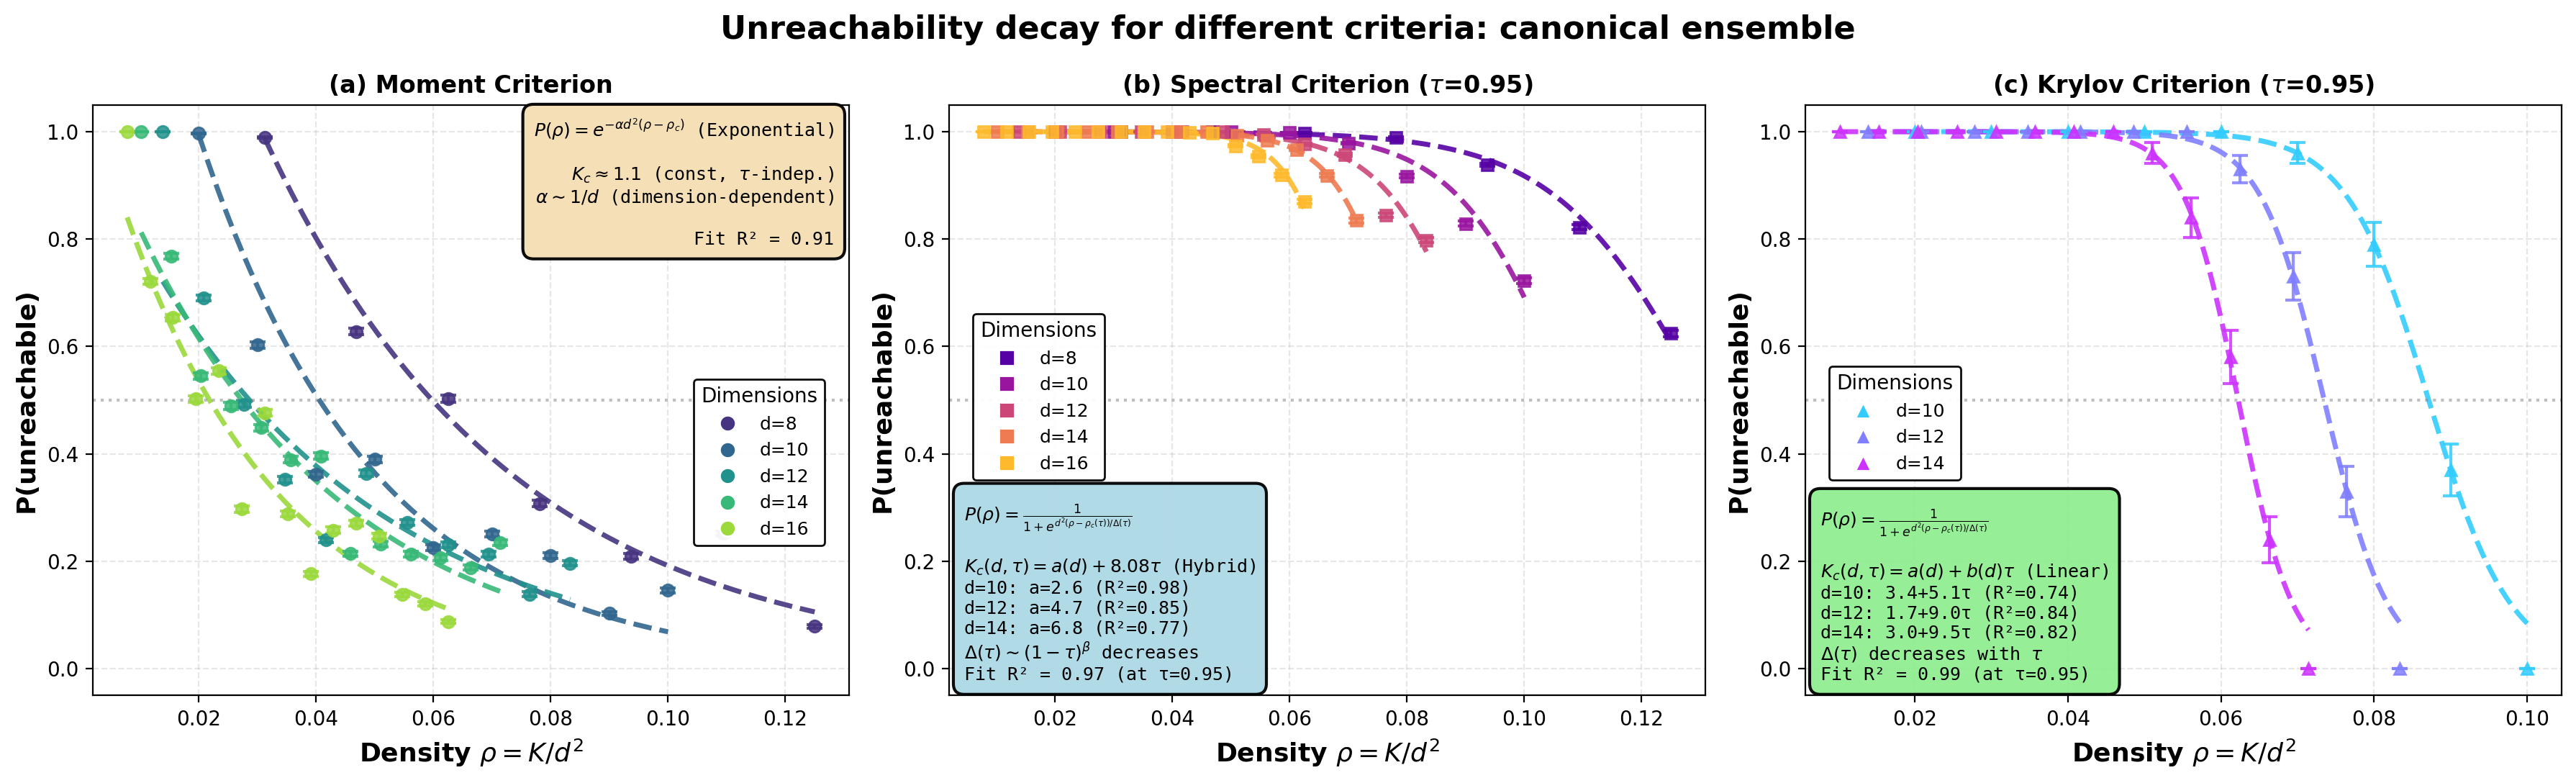
\includegraphics[width=0.99\textwidth]{fig/final_summary_P_vs_rho.png}
    \caption{Unreachability probability $P(\rho)$ versus control density $\rho = K/d^2$ for canonical basis ensemble. \textbf{(a) Moment:} Exponential decay \textbf{(b) Spectral:} Fermi-Dirac transition, $K_c(d,\tau) = a(d) + 8.08\tau$ . \textbf{(c) Krylov:} Linear $K_c(d,\tau) = a(d) + b(d)\tau$ with dimension-dependent slope ($b = 5.1$--$9.5$) (WHY??????). All criteria exhibit $\rho_c \sim 1/d$ scaling. \ph{It would be super useful to have the same x axis and colours for each dimension for comparison :), then you can do a single dimension legend at the bottom}}
    \label{fig:final_summary}
\end{figure*}

\begin{figure*}[!t]
    \centering
    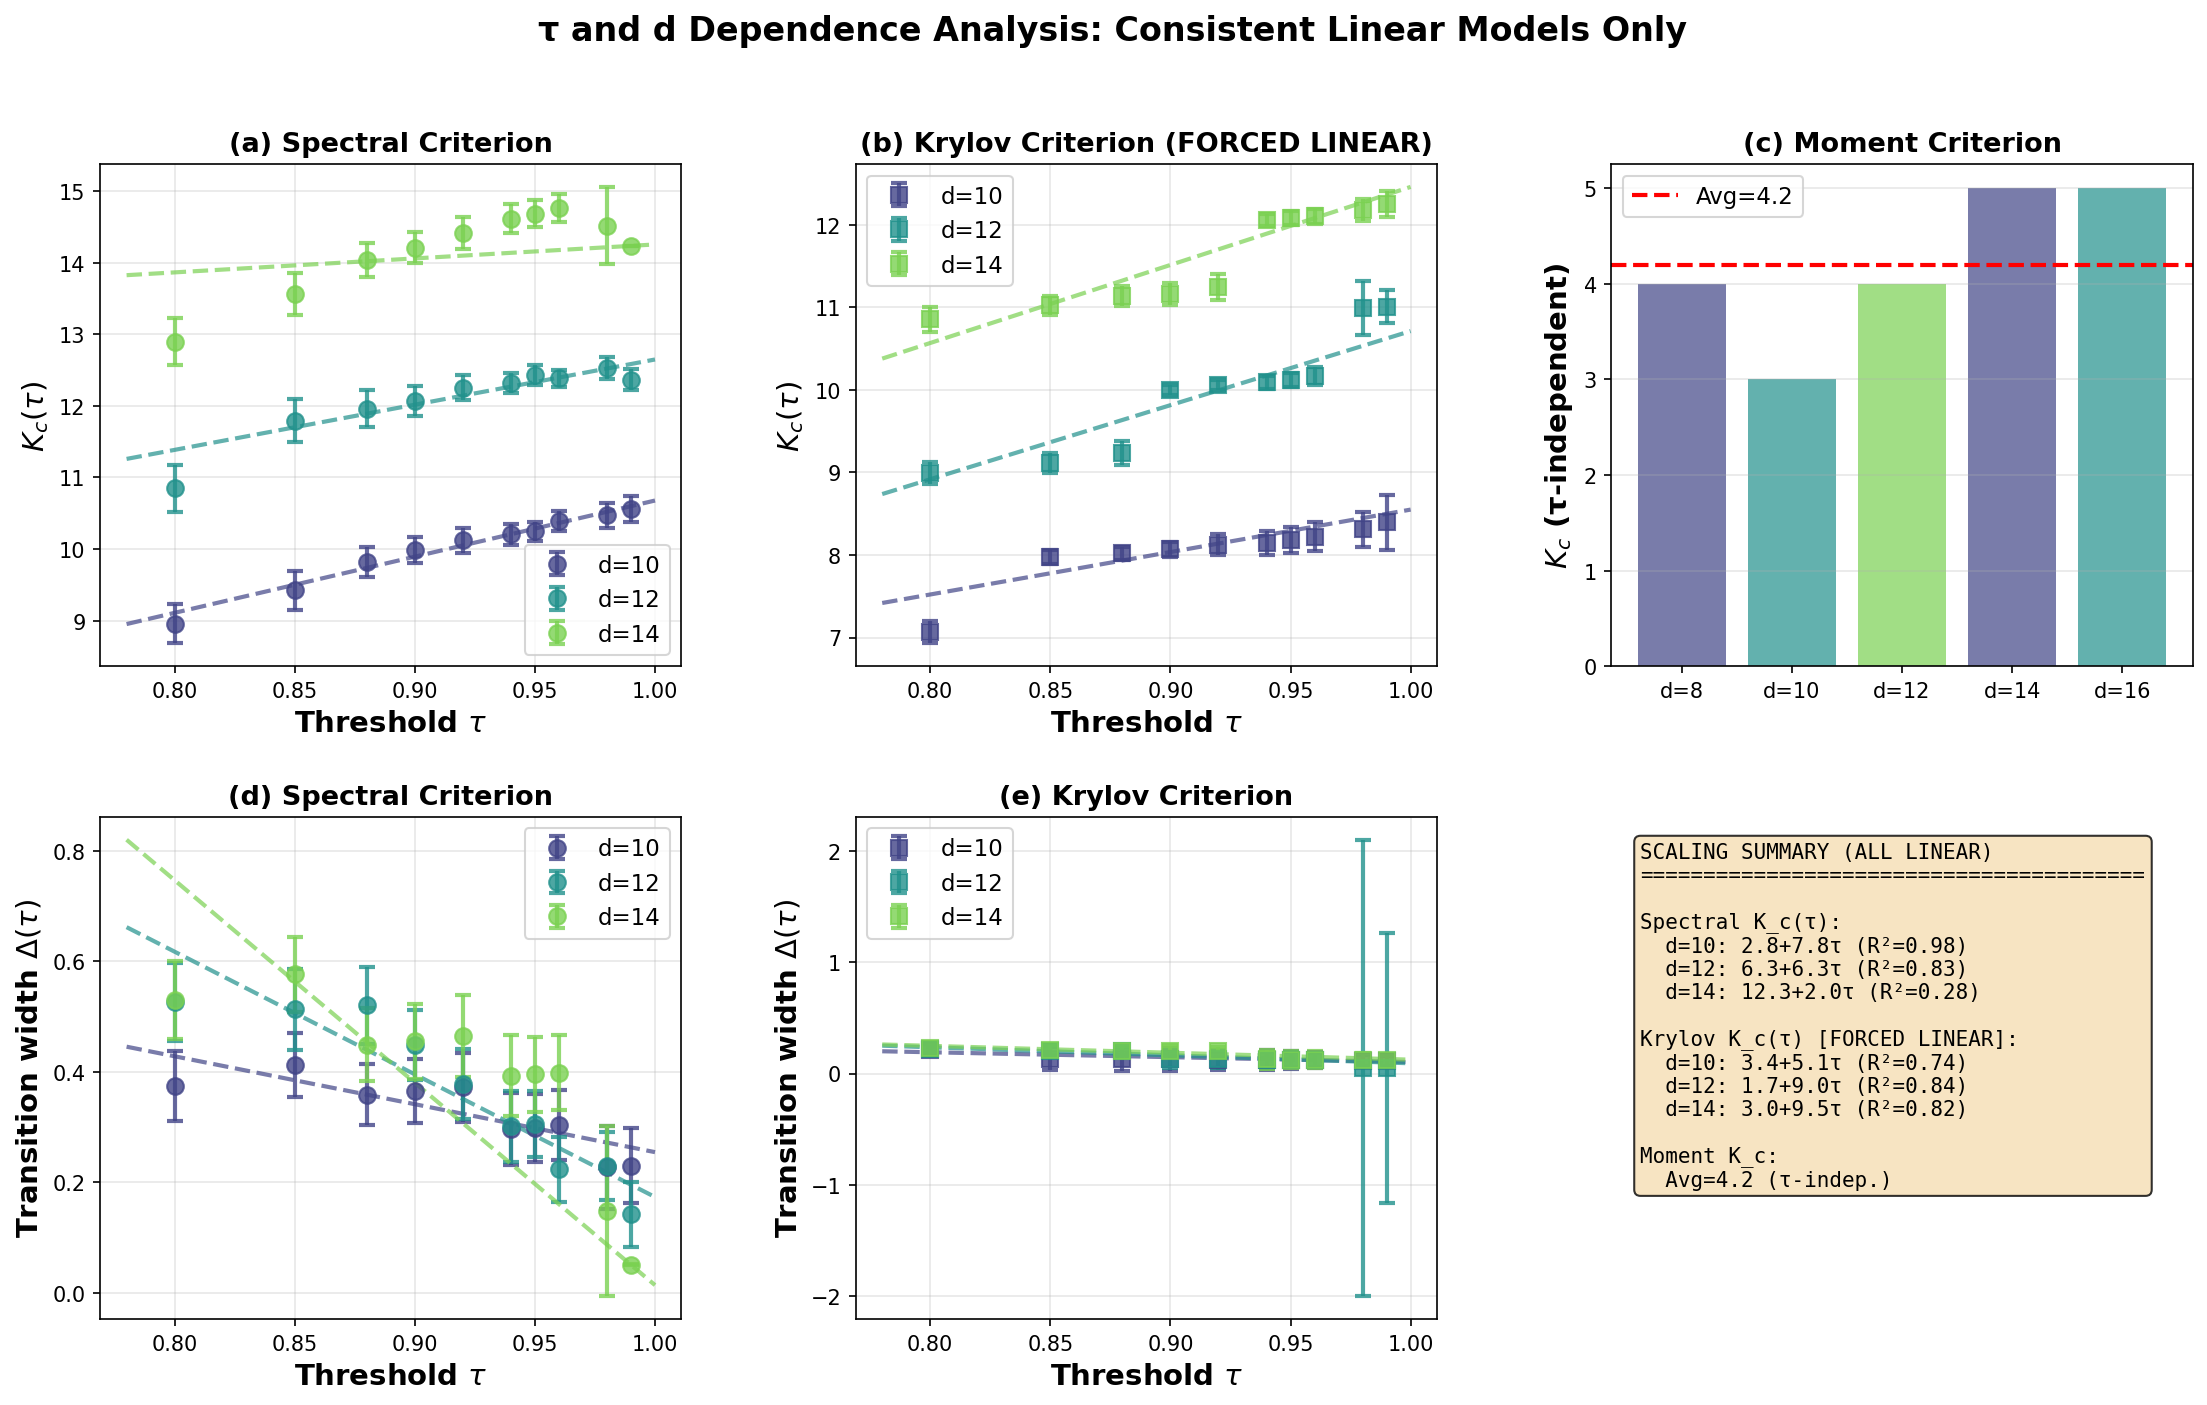
\includegraphics[width=0.95\textwidth]{fig/tau_d_comprehensive_analysis.png}
    \caption{$\tau$ and $d$ dependence analysis. \textbf{Top row:} Critical control number $K_c(\tau)$ increases linearly with threshold $\tau$ for both spectral criterion (universal slope $b \approx 8.08 \pm 0.35$) and Krylov criterion (dimension-dependent slopes $b = 5.1$--$9.5$) (WHY???). For moment criterion shows $K_c \approx 4.2$. \textbf{Bottom row:} Transition width $\Delta(\tau)$ decreases with $\tau$, following power-law $\Delta \sim (1-\tau)^\beta$ for spectral. Krylov exhibits smaller $\Delta$ than Spectral at fixed $\tau=0.95$.}
    \label{fig:tau_analysis}
\end{figure*}


\begin{figure}[!h]
    \centering
    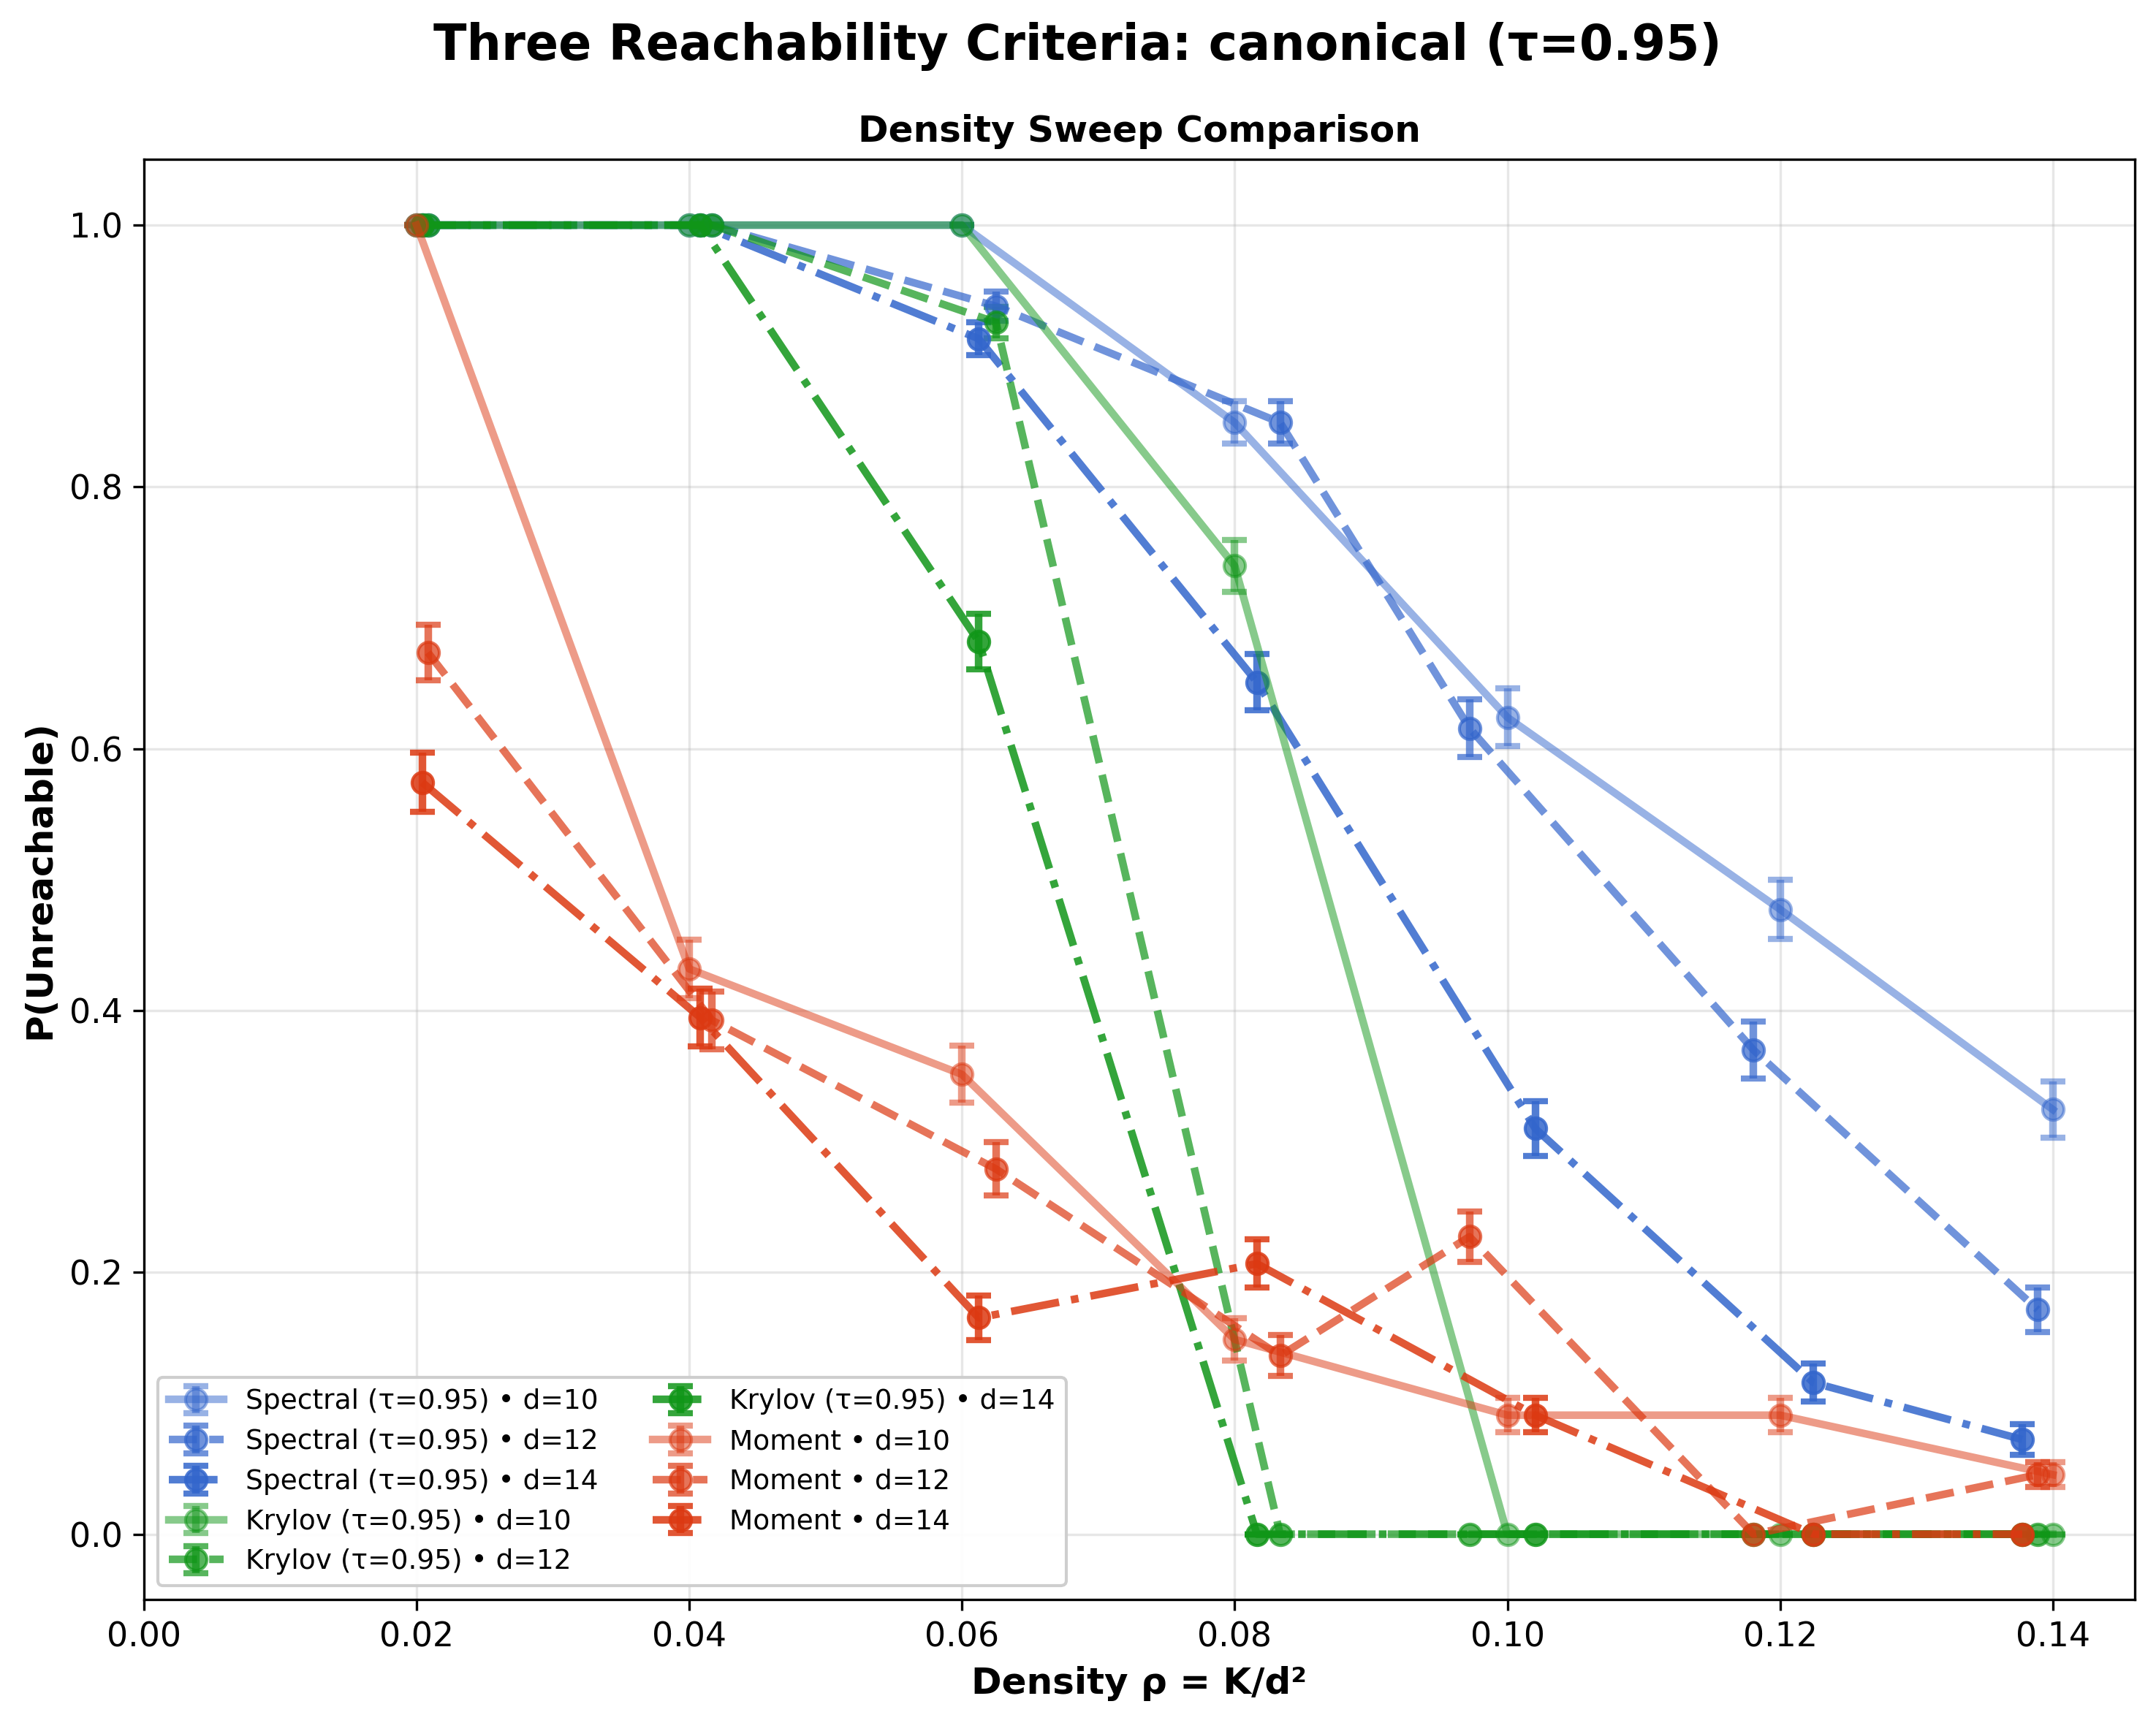
\includegraphics[width=0.9\linewidth]{fig/three_criteria_vs_density_canonical_tau0.95_unreachable.png}
    \caption{Probability of unreachability (according to 3 criteria  vs density for canonical ensemble}
    \label{fig:hilbert}
\end{figure}
\begin{figure}[!t]
    \centering
    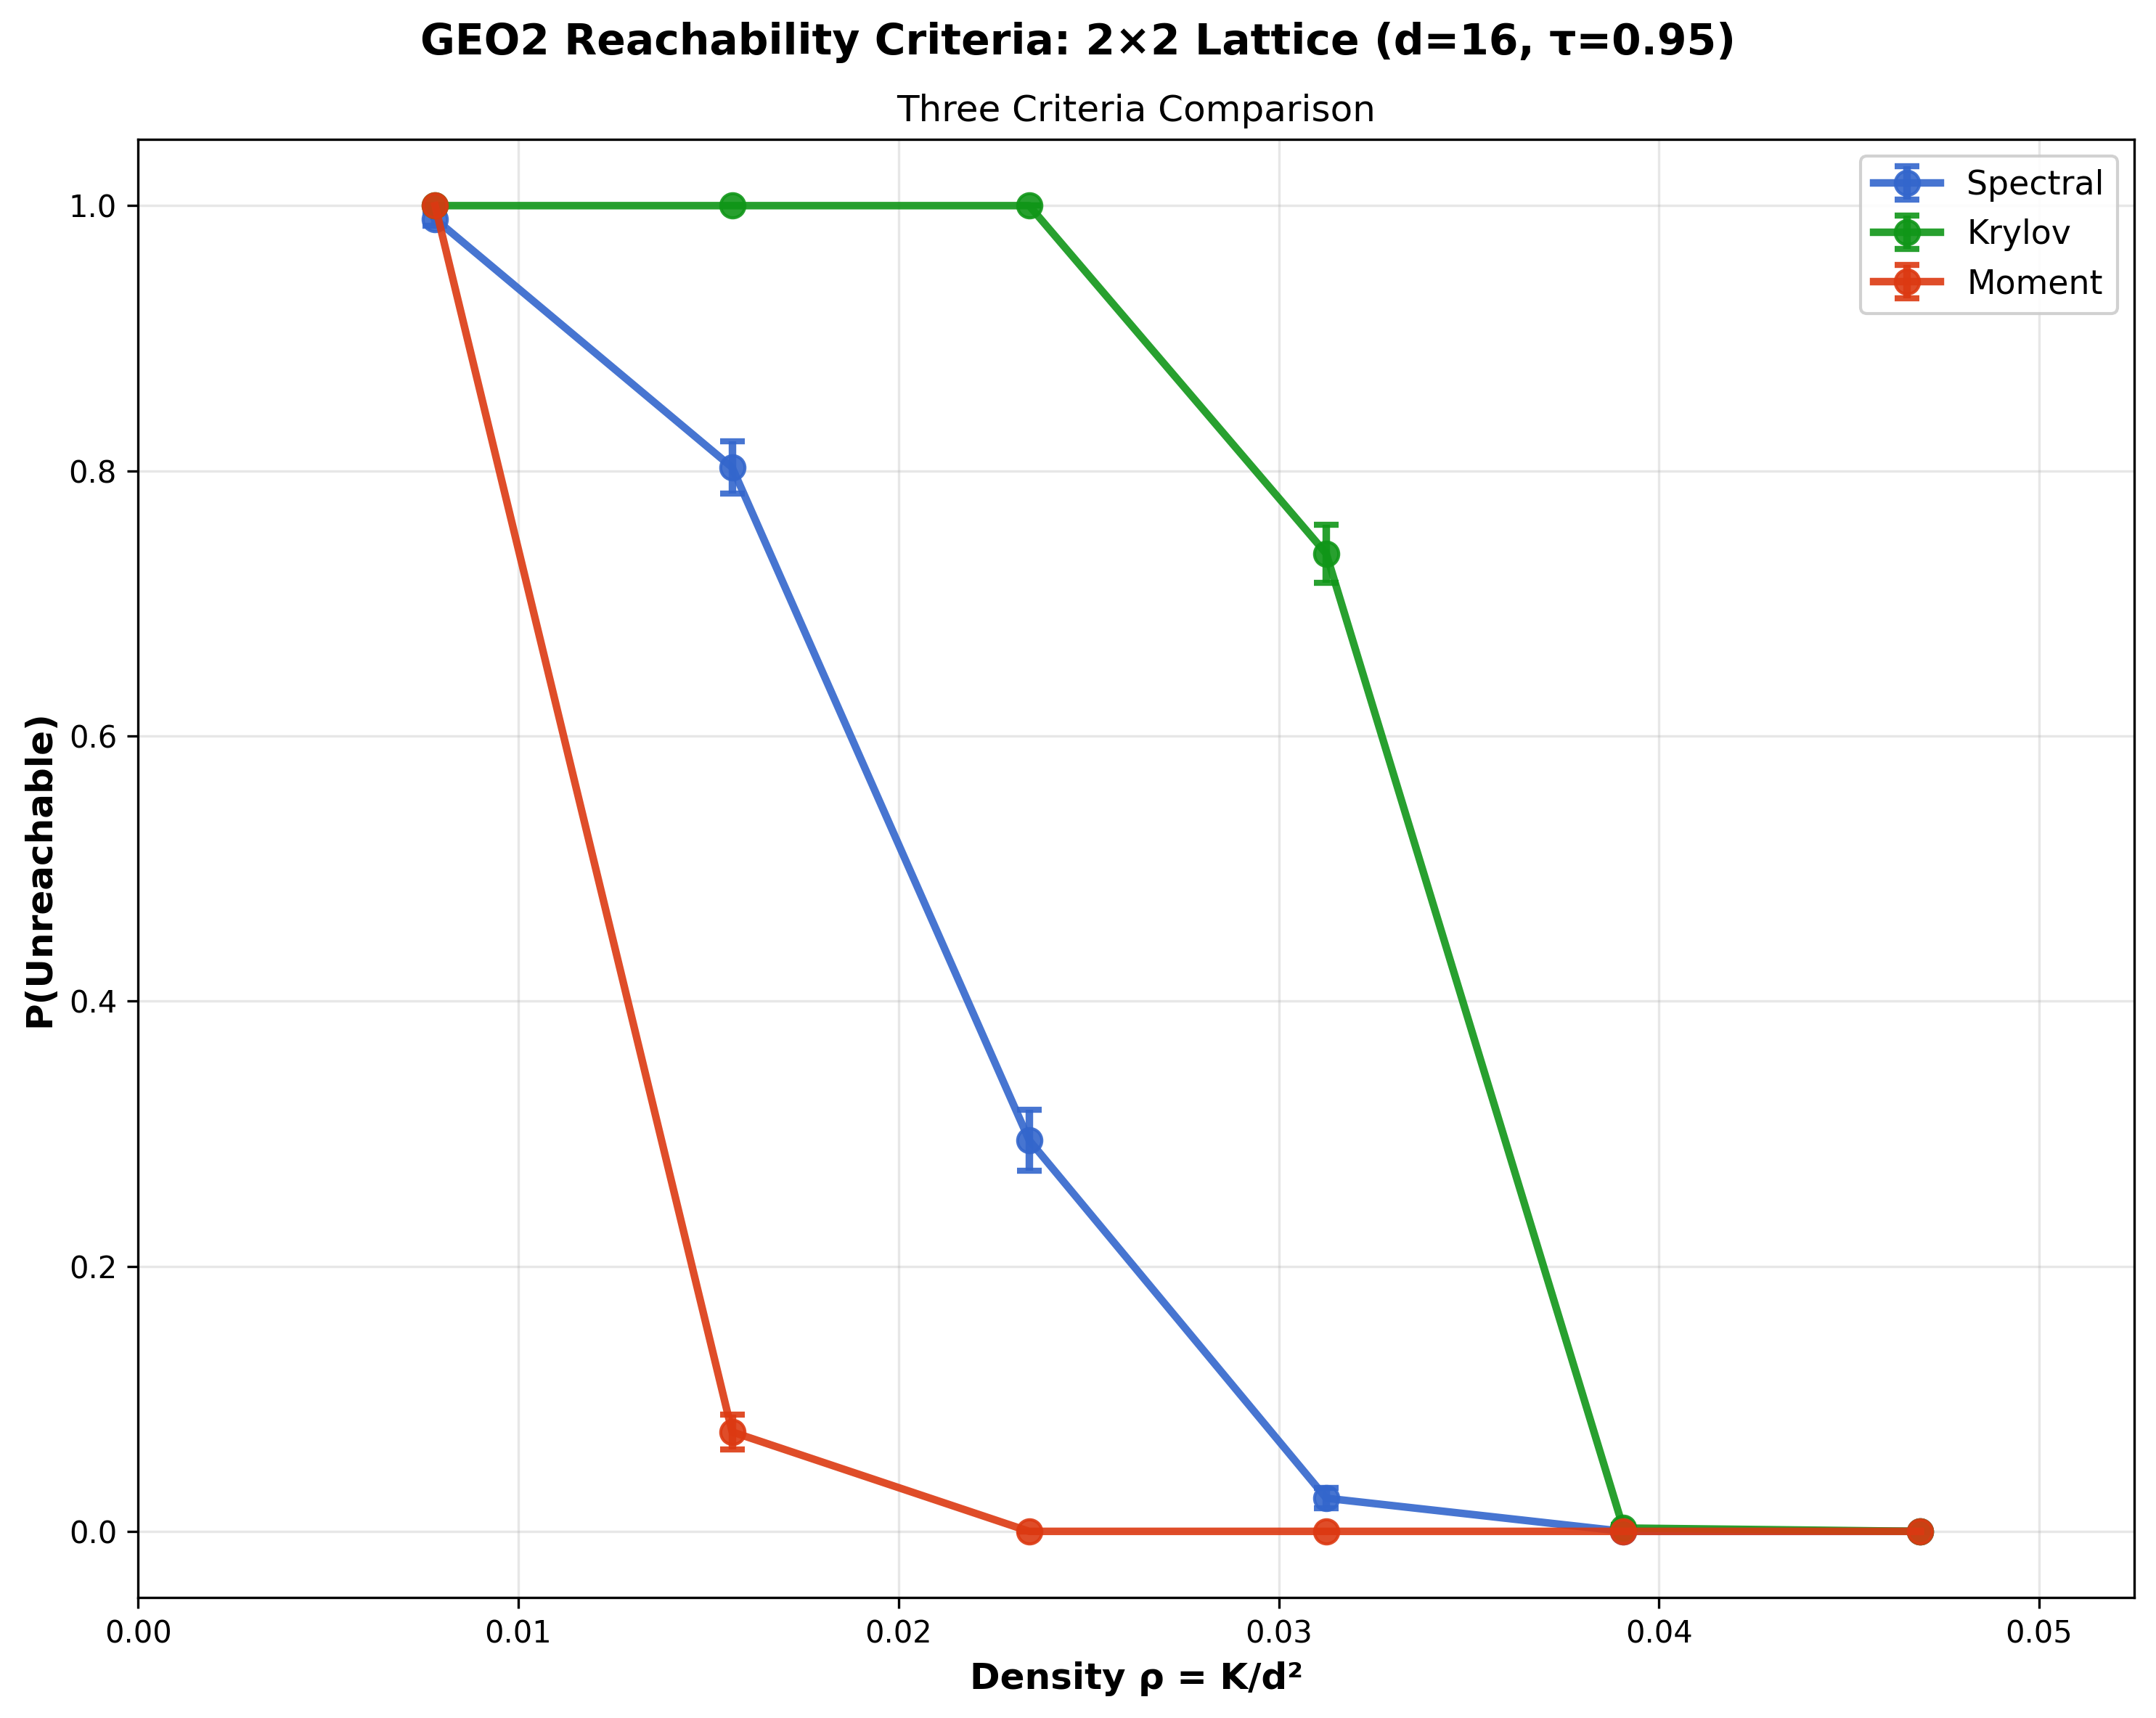
\includegraphics[width=0.9\linewidth]{fig/geo2_2x2_d16_publication.png}
    \caption{Probability of unreachability (according to 3 criteria  vs density for Geometric 2 local ensemble}
    \label{fig:hilbert2}
\end{figure}




\section{Bullshit}
\subsection{Where's the scaling coming from}


\bibliography{references}

\end{document}
